\documentclass[11pt,a4paper]{article}

% Tipografía y Lenguaje
\usepackage{fontspec}
\setmainfont{Georgia}[
  BoldFont={Georgia Bold},
  ItalicFont={Georgia Italic},
  BoldItalicFont={Georgia Bold Italic}
]
\usepackage[spanish,es-tabla]{babel}

% Geometría de Página
\usepackage[top=2.5cm, bottom=2.5cm, left=2.5cm, right=2.5cm, headheight=22pt]{geometry}

% Paquetes Matemáticos y Tablas
\usepackage{amsmath, amsfonts, amssymb}
\usepackage{booktabs}
\usepackage{graphicx}
\usepackage{float}
\usepackage{xcolor}
\usepackage{microtype}
\usepackage{setspace}
\usepackage{fancyhdr}
\usepackage{caption}

% Rutas de Figuras
\graphicspath{{../04_Figuras/}}

% Paleta Cromática Académica
\definecolor{navyblue}{HTML}{1A2B4C}
\definecolor{darkslate}{HTML}{2F3E46}
\definecolor{accentblue}{HTML}{2B6CB0}
\definecolor{lightborder}{HTML}{CBD5E0}

% Configuración de Hipervínculos
\usepackage[
  colorlinks=true,
  linkcolor=navyblue,
  citecolor=accentblue,
  urlcolor=accentblue,
  pdfauthor={Federico Agustín Chillón},
  pdftitle={Optimización de Portafolios: Markowitz, HERC, Modelización de Riesgos y Backtesting}
]{hyperref}
\usepackage{bookmark}

% Configuración de Leyendas
\captionsetup{
  font={small,stretch=1.15},
  labelfont={bf,color=navyblue},
  textfont={it},
  justification=justified,
  singlelinecheck=false,
  skip=6pt
}

% Encabezados y Pies de Página
\pagestyle{fancy}
\fancyhf{}
\renewcommand{\headrulewidth}{0.4pt}
\renewcommand{\headrule}{\hbox to\headwidth{\color{lightborder}\leaders\hrule height \headrulewidth\hfill}}
\fancyhead[L]{\footnotesize\color{darkslate}\textit{Optimización de Portafolios y Contrastación Empírica}}
\fancyhead[R]{\footnotesize\color{darkslate}\textit{F. A. Chillón (2026)}}
\fancyfoot[C]{\footnotesize\color{darkslate}\thepage}

% Formato de Secciones APA 7
\makeatletter
\renewcommand\section{\@startsection{section}{1}{\z@}%
  {16pt \@plus 3pt \@minus 2pt}%
  {6pt}%
  {\centering\large\bfseries\color{navyblue}}}
\renewcommand\subsection{\@startsection{subsection}{2}{\z@}%
  {12pt \@plus 2pt \@minus 1pt}%
  {4pt}%
  {\raggedright\normalsize\bfseries\color{navyblue}}}
\renewcommand\subsubsection{\@startsection{subsubsection}{3}{\z@}%
  {10pt \@plus 2pt \@minus 1pt}%
  {3pt}%
  {\raggedright\normalsize\bfseries\itshape\color{navyblue}}}
\makeatother

% Control de Líneas Huérfanas y Viudas
\widowpenalty=10000
\clubpenalty=10000

% Tipografía y Espaciado
\setstretch{1.22}
\setlength{\parindent}{1.25em}
\setlength{\parskip}{2pt}

\begin{document}

% ==================== PORTADA (PÁGINA 1) ====================
\begin{titlepage}
\thispagestyle{empty}
\centering
\vspace*{3.5cm}

{\LARGE \textbf{\color{navyblue}Optimización de Portafolios:\\[0.35cm] Markowitz, HERC, Modelización de Riesgos y Backtesting}}\\[0.8cm]

{\large \textit{\color{darkslate}Evaluación Empírica y Contrastación de Modelos de Asignación de Activos (2007--2026)}}\\[5.0cm]

\vfill

{\normalsize \textbf{Autor}}\\[0.2cm]
{\Large \textbf{\color{navyblue}Federico Agustín Chillón}}\\[0.4cm]
{\normalsize \color{darkslate}Investigación Cuantitativa y Gestión de Portafolios}\\[0.2cm]
{\small \color{darkslate}Mendoza, Argentina \textbar\ Agosto de 2026}
\vspace*{2.0cm}

\end{titlepage}

% ==================== PÁGINA 2: DESCARGO ====================
\newpage
\thispagestyle{empty}

\vspace*{2cm}
\begin{center}
{\large\bfseries\color{navyblue} Declaración de Divulgación y Descargo de Responsabilidad}
\end{center}
\vspace{0.4cm}

\begingroup
\setlength{\parindent}{0pt}
\small\color{darkslate}
Este trabajo ha sido elaborado con propósitos estrictamente académicos. Los modelos analíticos, algoritmos de optimización, contrastes econométricos y resultados de simulación retrospectiva (\textit{backtesting}) presentados no constituyen asesoramiento financiero, consultoría de inversiones, gestión fiduciaria ni solicitud u oferta de compra o venta de instrumentos financieros, fondos cotizados (ETFs) o valores negociables.

\vspace{0.4cm}
El desempeño histórico fuera de muestra no garantiza resultados futuros. Toda implementación práctica de modelos de asignación de capital está sujeta a riesgos de mercado, deslizamiento en la ejecución y variaciones en la liquidez de los activos subyacentes.
\endgroup

\vfill
\noindent{\footnotesize\color{darkslate}\textit{Documento técnico de investigación | Investigación Cuantitativa | Mendoza, Argentina}}

% ==================== PÁGINA 3: ÍNDICE ====================
\newpage
\thispagestyle{empty}

\vspace*{1cm}
\begin{center}
{\large\bfseries\color{navyblue} Índice General}
\end{center}
\vspace{0.2cm}

\begin{spacing}{1.08}
\small
\makeatletter
\@starttoc{toc}
\makeatother
\end{spacing}

% ==================== RESUMEN (APA 7 - PÁGINA 3) ====================
\newpage
\pagenumbering{arabic}

\begin{center}
\textbf{\large\color{navyblue} Resumen}
\end{center}
\vspace{0.2cm}

\noindent Se examina el desempeño fuera de muestra de nueve modelos de asignación de activos sobre nueve ETFs líquidos entre 2007 y 2026. La comparación incluye la cartera de referencia 60/40, la cartera equiponderada (1/N), carteras clásicas de media-varianza (Markowitz MVO y Markowitz Remuestreado por Bootstrap), modelos de riesgo de cola (Mín. CVaR y Mín. CDaR), el algoritmo HERC, la Optimización Distribucionalmente Robusta con métrica de Wasserstein (Esfahani y Kuhn, 2018) y el Marco Generativo Ex-Ante GARCH-EVT-Cópula (Barone-Adesi et al., 1999; McNeil et al., 2015; Patton, 2012). El diseño combina un protocolo \textit{Walk-Forward} con deriva diaria de precios, costos de transacción de 5 puntos básicos, medición de pérdidas extremas con Teoría de Valores Extremos (Pareto Generalizada), Validación Cruzada Combinatoria con Embargo (CPCV) y pruebas de significancia con Probabilistic Sharpe Ratio (PSR) y Deflated Sharpe Ratio (DSR). Los resultados indican que ningún modelo domina al resto en todas las métricas: la cartera 60/40 obtiene el mayor CAGR neto (9.64\%) y el Sharpe más alto (0.78), Markowitz MVO alcanza el mayor retorno acumulado absoluto (495.64\%), Mín-CVaR la pérdida más baja en eventos de cola, HERC la diversificación efectiva más alta entre los modelos sin robustez distribucional explícita ($N_{\text{eff}} = 6.46$) y DRO-Wasserstein la rotación más baja de todo el estudio (3.77\%).\\[0.35cm]
\indent \textit{Palabras clave:} Asignación de activos, HERC, Markowitz, retroceso condicional, Teoría de Valores Extremos, Validación Cruzada Combinatoria, Probabilistic Sharpe Ratio.\\[0.2cm]
\indent \textit{Clasificación JEL:} C58, C61, G11, G14. \quad \textit{MSC (2020):} 91G10, 90C90, 62P05.

\vspace{0.5cm}

% ==================== CUERPO DEL TRABAJO ====================

\section{Marco Conceptual y Límites de Media-Varianza}

La teoría clásica de selección de carteras (Markowitz, 1952) formula la asignación de capital como la maximización de la utilidad cuadrática esperada:
\begin{equation}
\max_{w} \quad \mu^T w - \frac{\gamma}{2} w^T \Sigma w \quad \text{sujeto a} \quad \mathbf{1}^T w = 1, \quad w_i \ge 0 \quad \forall i
\end{equation}
Aquí $\mu \in \mathbb{R}^N$ es el vector de rendimientos esperados, $\Sigma \in \mathbb{R}^{N \times N}$ la matriz de covarianza poblacional, $\gamma > 0$ el coeficiente de aversión al riesgo y $w \in \mathbb{R}^N$ el vector de ponderaciones. En este trabajo se fija $\gamma = 2.5$, un valor habitual para gestión moderada en asignación multiactivo.

Estimar $\mu$ y $\Sigma$ directamente de la muestra tiene limitaciones prácticas serias. Michaud (1989) demostró que el optimizador de media-varianza actúa como amplificador de errores muestrales (\textit{error maximizer}). Los activos con rendimientos sobrestimados o varianzas subestimadas reciben ponderaciones desproporcionadas. Por eso las carteras óptimas tienden a concentrarse en pocos instrumentos y muestran alta inestabilidad temporal, lo que induce rotaciones excesivas.

Además, la varianza penaliza por igual las desviaciones positivas y negativas. Ese supuesto no se cumple en distribuciones con asimetría negativa y colas pesadas, donde la varianza subestima el riesgo de eventos extremos.

Para reducir el error de estimación de la matriz de covarianza sin imponer restricciones paramétricas rígidas se usa el estimador de contracción lineal (\textit{shrinkage}) de Ledoit y Wolf (2004). Ese estimador combina la matriz muestral $S$ con una estructura objetivo $F$ de correlación constante:
\begin{equation}
\Sigma_{\text{LW}} = \hat{\delta} F + (1 - \hat{\delta}) S
\end{equation}
La intensidad de contracción $\hat{\delta} \in [0, 1]$ se determina analíticamente minimizando la pérdida cuadrática esperada bajo la norma de Frobenius. Para $A \in \mathbb{R}^{N \times N}$, esa norma se define como:
\begin{equation}
\|A\|_F = \sqrt{\sum_{i=1}^{N} \sum_{j=1}^{N} a_{ij}^2} = \sqrt{\operatorname{tr}\left(A^\top A\right)}
\end{equation}
Ledoit y Wolf (2004) minimizan $\mathbb{E}\left[\left\|\Sigma_{\text{LW}} - \Sigma_0\right\|_F^2\right]$ respecto de $\hat{\delta}$, donde $\Sigma_0$ es la matriz de covarianza poblacional desconocida.

\section{Universo Multiactivo y Topología de Dependencias}

El universo analizado comprende 9 fondos cotizados (ETFs) seleccionados por su representatividad macroeconómica y liquidez continua entre enero de 2007 y agosto de 2026 ($T = 4\,928$ ruedas):
\begin{itemize}
    \item Renta Variable EE.UU.: SPY (S\&P 500) y QQQ (Nasdaq 100).
    \item Renta Variable Mercados Emergentes: EEM (MSCI Emerging Markets).
    \item Bienes Raíces e Infraestructura: VNQ (Vanguard Real Estate).
    \item Renta Fija Soberana EE.UU.: TLT (Tesoro 20+ Años) e IEF (Tesoro 7--10 Años).
    \item Renta Fija Corporativa Grado de Inversión: LQD (iShares Investment Grade Corporate Bond).
    \item Metales Preciosos: GLD (SPDR Gold Shares).
    \item Materias Primas: DBC (Invesco DB Commodity Index Tracking Fund).
\end{itemize}

La correlación lineal $\rho_{ij}$ se convierte en una distancia métrica angular con la fórmula:
\begin{equation}
d_{ij} = \sqrt{0.5 \left(1 - \rho_{ij}\right)}
\end{equation}
La matriz $D = (d_{ij})$ cumple las propiedades métricas euclidianas. Sobre esa matriz se ejecuta un agrupamiento jerárquico aglomerativo con enlace de Ward, que fusiona grupos de forma recursiva minimizando el incremento en la suma de cuadrados de las distancias internas:
\begin{equation}
\Delta \text{ESS}(A, B) = \frac{|A| |B|}{|A| + |B|} \|\bar{x}_A - \bar{x}_B\|^2
\end{equation}
Al reordenar la matriz de correlación según el dendrograma se observan los bloques homogéneos de covariación del mercado (Figura~\ref{fig:dendrograma}).

\begin{figure}[H]
\centering
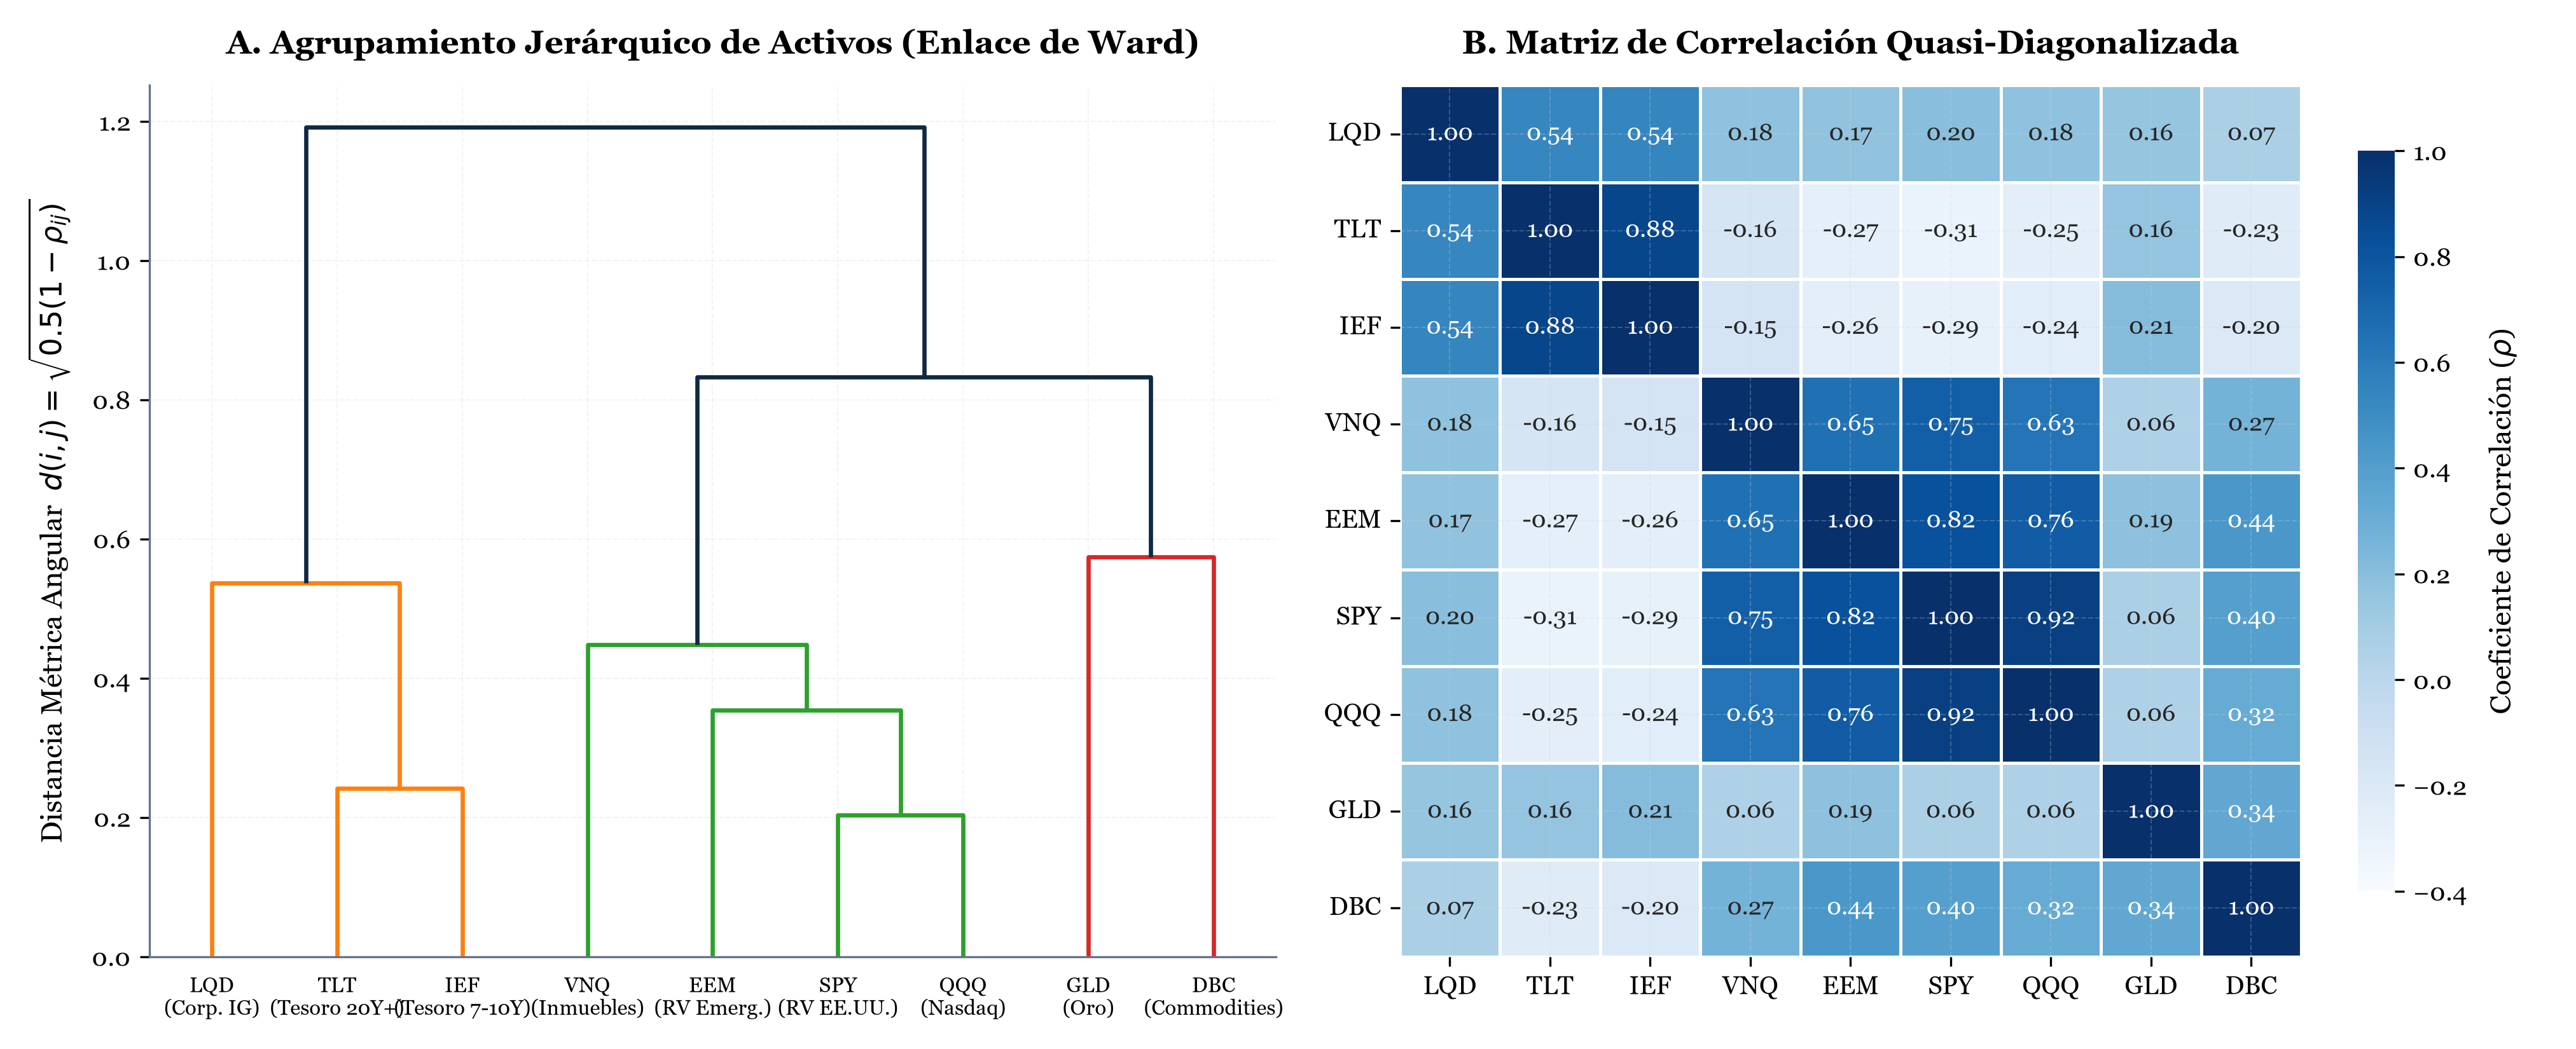
\includegraphics[width=0.92\textwidth]{fig01_dendrograma_correlaciones.png}
\caption{Dendrograma de agrupamiento jerárquico de activos bajo enlace de Ward y matriz de correlación reordenada.}
\label{fig:dendrograma}
\end{figure}

\subsection{Diagnóstico Econométrico y Validación de Supuestos Estadísticos}

La Tabla~\ref{tab:diagnostico} resume las propiedades estadísticas de las $4\,928$ ruedas históricas del universo de activos.

\begin{table}[H]
\centering
\renewcommand{\arraystretch}{1.15}
\caption{Diagnóstico econométrico y contrastes de hipótesis sobre las series temporales de activos (2007--2026).}
\label{tab:diagnostico}
\resizebox{\textwidth}{!}{%
\begin{tabular}{llrrrrrrrr}
\toprule
\textbf{Ticker} & \textbf{Clase de Activo} & \textbf{Ret. Anual (\%)} & \textbf{Vol. Anual (\%)} & \textbf{Asimetría} & \textbf{Exceso Curt.} & \textbf{JB ($p$-val)} & \textbf{Ljung-Box $Q(10)$} & \textbf{ARCH-LM $Q(10)$} & \textbf{ADF Ret. ($p$-val)} \\
\midrule
SPY & Renta Variable EE.UU. & 10.35 & 19.63 & $-0.30$ & $+13.92$ & $< 10^{-4}$ & $< 10^{-14}$ & $< 10^{-4}$ & $< 10^{-27}$ \\
QQQ & Renta Variable Tecnológica & 14.95 & 22.26 & $-0.26$ & $+7.29$ & $< 10^{-4}$ & $< 10^{-13}$ & $< 10^{-4}$ & $< 10^{-29}$ \\
EEM & Renta Variable Emergente & 4.68 & 27.99 & $+0.03$ & $+16.12$ & $< 10^{-4}$ & $< 10^{-15}$ & $< 10^{-4}$ & $< 10^{-23}$ \\
VNQ & Bienes Raíces (REITs) & 5.42 & 29.58 & $-0.52$ & $+17.87$ & $< 10^{-4}$ & $< 10^{-15}$ & $< 10^{-4}$ & $< 10^{-25}$ \\
TLT & Renta Fija Soberana (20Y+) & 2.71 & 15.05 & $+0.01$ & $+3.20$ & $< 10^{-4}$ & $< 10^{-5}$ & $< 10^{-4}$ & $< 10^{-24}$ \\
IEF & Renta Fija Soberana (7--10Y) & 3.14 & 6.92 & $+0.12$ & $+2.59$ & $< 10^{-4}$ & $0.0048$ & $< 10^{-4}$ & $< 10^{-30}$ \\
LQD & Renta Fija Crédito IG & 3.94 & 8.79 & $-0.45$ & $+56.88$ & $< 10^{-4}$ & $< 10^{-15}$ & $< 10^{-4}$ & $< 10^{-24}$ \\
GLD & Metales Preciosos (Oro) & 9.14 & 18.15 & $-0.43$ & $+7.08$ & $< 10^{-4}$ & $0.4678$ & $< 10^{-4}$ & $< 10^{-30}$ \\
DBC & Materias Primas & 2.15 & 19.35 & $-0.49$ & $+3.35$ & $< 10^{-4}$ & $0.9888$ & $< 10^{-4}$ & $< 10^{-30}$ \\
\bottomrule
\end{tabular}%
}
\end{table}

Los resultados de los contrastes son los siguientes:
\begin{enumerate}
    \item \textbf{No normalidad de los rendimientos.} El test de Jarque y Bera (1980) rechaza la normalidad en todos los activos ($p < 0.0001$). Las series presentan leptocurtosis, con curtosis de exceso de $+56.88$ en LQD y $+17.87$ en VNQ, y asimetría negativa en general.
    \item \textbf{Heterocedasticidad condicional y efectos ARCH.} El estadístico $Q(10)$ de Ljung-Box sobre rendimientos al cuadrado ($r_t^2$) da $p < 0.0001$ en todos los activos. Eso confirma agrupamiento de volatilidad (\textit{volatility clustering}) y descarta el supuesto de varianza constante en retornos brutos (Engle, 1982).
    \item \textbf{Estacionariedad.} El test ADF confirma que los log-precios son integrados $I(1)$ con $p > 0.05$, mientras que los rendimientos logarítmicos continuos son estacionarios $I(0)$ con $p < 10^{-20}$.
    \item \textbf{Condicionamiento matricial.} La matriz muestral $S$ tiene número de condición $\kappa(S) = 335.21$. La contracción de Ledoit-Wolf lo reduce a $\kappa(\Sigma_{\text{LW}}) = 241.06$, con autovalor mínimo $\lambda_{\min} = 8.82 \times 10^{-4} > 0$.
\end{enumerate}

\section{Metodología de Modelos de Asignación}

Todas las estrategias imponen no negatividad ($w_i \ge 0$) y presupuesto unitario ($\sum_{i=1}^N w_i = 1$).

\subsection{Asignación Equiponderada (1/N) y Cartera de Referencia 60/40}

La cartera 1/N fija $w_i = 1/9$ en cada fecha de rebalanceo. La cartera 60/40 mantiene $w_{\text{SPY}} = 0.60$ e $w_{\text{IEF}} = 0.40$.

\subsection{Markowitz Media-Varianza}

Resuelve el problema cuadrático clásico con $\gamma = 2.5$ usando rendimientos anualizados y la matriz $\Sigma_{\text{LW}}$.

\subsection{Markowitz Remuestreado por Bootstrap}

Siguiendo a Michaud (1989), se generan $B = 25$ remuestreos bootstrap con reemplazo. En cada réplica $b$, se calculan los parámetros $(\mu_b, \Sigma_b)$, se obtiene el vector óptimo $w_b^{\text{opt}}$ y se computa el promedio de las asignaciones:
\begin{equation}
w_{\text{Michaud}} = \frac{1}{B} \sum_{b=1}^B w_b^{\text{opt}}
\end{equation}

\subsection{Mínimo Valor en Riesgo Condicional (CVaR)}

La minimización del CVaR al nivel de confianza $\alpha = 0.95$ (Rockafellar y Uryasev, 2000, 2002) se formula como un problema de programación lineal con variables auxiliares $z_t$:
\begin{equation}
\min_{w, \zeta, z} \quad \zeta + \frac{1}{T(1-\alpha)} \sum_{t=1}^T z_t \quad \text{sujeto a} \quad z_t \ge -r_t^T w - \zeta, \quad z_t \ge 0, \quad \mathbf{1}^T w = 1, \quad w \ge 0
\end{equation}
El escalar $\zeta \in \mathbb{R}$ es el estimador del VaR y $z_t$ mide los excesos de pérdida por encima de ese nivel.

\subsection{Mínimo Retroceso Condicional Acumulado (CDaR)}

El modelo de Chekhlov, Uryasev y Zabarankin (2005) optimiza la trayectoria temporal de caídas respecto al pico histórico. Sea $W_t(w) = \sum_{s=1}^t r_s^T w$ el retorno acumulado y $M_t(w) = \max_{0 \le s \le t} W_s(w)$ el máximo alcanzado hasta la rueda $t$. El retroceso o \textit{drawdown} se define como $D_t(w) = M_t(w) - W_t(w) \ge 0$.

El CDaR al $95\%$ promedia el $5\%$ de las mayores caídas acumuladas. La optimización lineal se expresa mediante:
\begin{equation}
\min_{w, \nu, u, d} \quad \nu + \frac{1}{T (1 - \alpha)} \sum_{t=1}^T u_t
\end{equation}
sujeto a:
\begin{equation}
u_t \ge d_t - \nu, \quad u_t \ge 0, \quad d_t \ge M_t(w) - W_t(w), \quad d_t \ge 0, \quad \mathbf{1}^T w = 1, \quad w_i \ge 0
\end{equation}
El parámetro $\nu \in \mathbb{R}$ representa el umbral $\text{DaR}_{95\%}$ y $u_t$ cuantifica las pérdidas acumuladas que exceden ese umbral.

\subsection{Asignación Jerárquica de Contribución de Riesgo Equitativo (HERC)}

A diferencia de la Paridad de Riesgo Jerárquica tradicional (HRP; López de Prado, 2016) basada en bisección por índices, HERC (Raffinot, 2017, 2018) preserva la estructura de clusters del enlace de Ward. En cada bifurcación entre dos grupos $C_1$ y $C_2$, el capital se distribuye en proporción inversa a la volatilidad agregada $\sigma_{C_k} = \sqrt{w_k^T \Sigma_{C_k} w_k}$:
\begin{equation}
\alpha_{C_1} = \frac{1 / \sigma_{C_1}}{1 / \sigma_{C_1} + 1 / \sigma_{C_2}}, \quad \alpha_{C_2} = 1 - \alpha_{C_1}
\end{equation}
Dentro de cada cluster, los pesos individuales se asignan por paridad inversa a su varianza ($1 / \sigma_i^2$). Este procedimiento distribuye el presupuesto de riesgo a lo largo del árbol sin invertir la matriz de covarianza completa. La Figura~\ref{fig:frontera} muestra en el Panel A la frontera eficiente analítica de Markowitz, los 9 activos individuales y la nube de 6\,000 carteras simuladas por Monte Carlo. El Panel B ilustra el cono de incertidumbre bajo remuestreo bootstrap, con intervalos de confianza al 80\% y 90\%, y la frontera promedio de Michaud.

\begin{figure}[H]
\centering
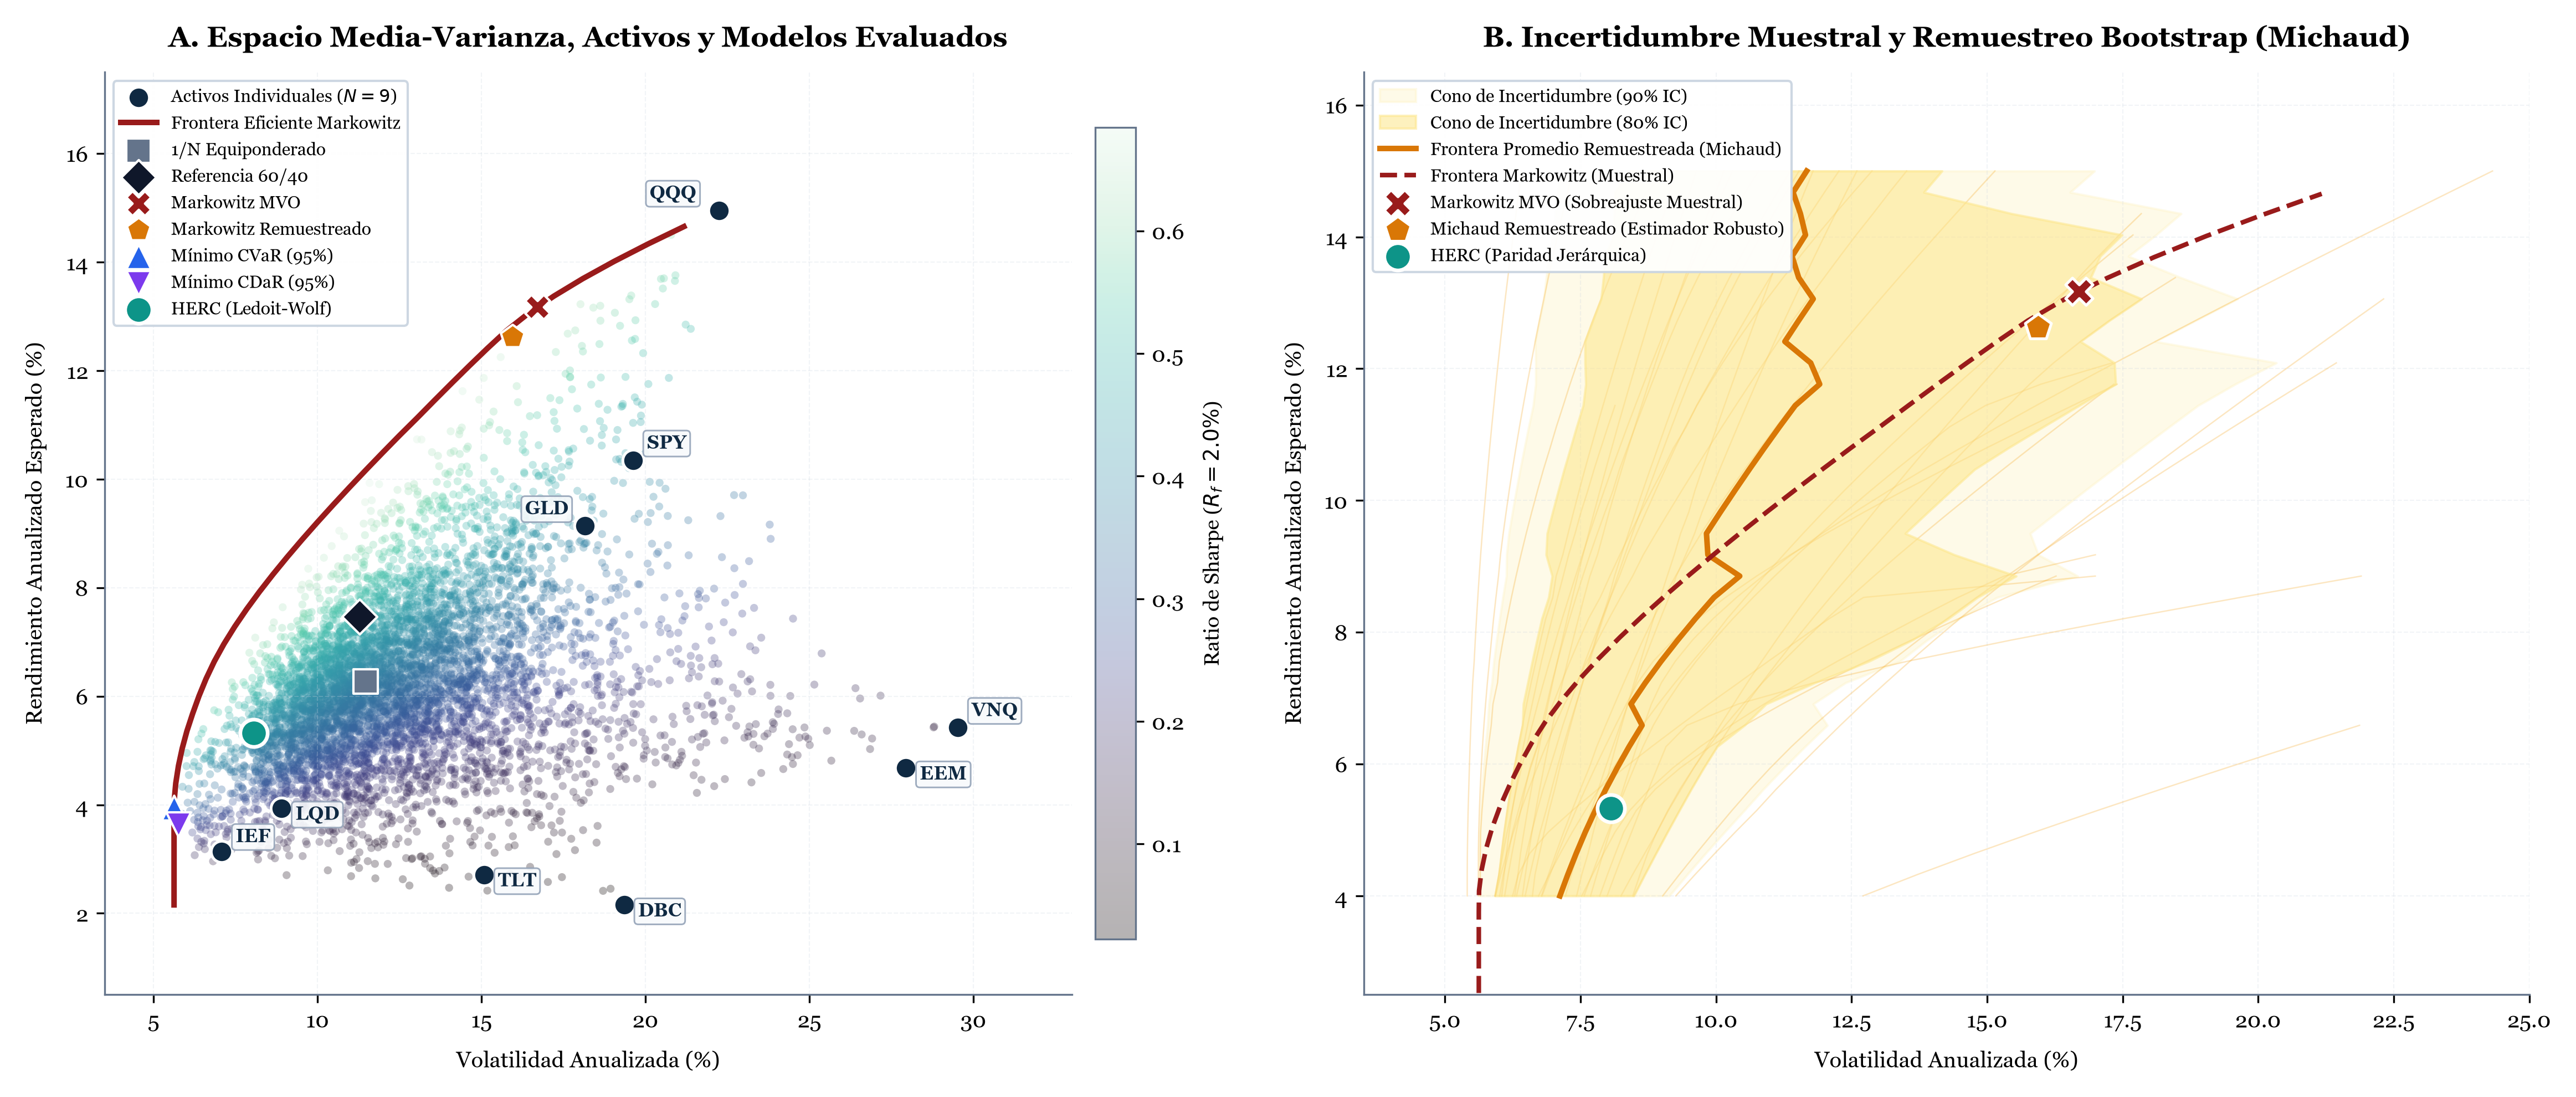
\includegraphics[width=0.96\textwidth]{fig02_frontera_eficiente_modelos.png}
\caption{Frontera eficiente media-varianza analítica, posicionamiento de activos y los nueve modelos evaluados en este documento --incluidos DRO-Wasserstein y Marco Generativo Ex-Ante-- (Panel A) y cono de incertidumbre muestral bajo remuestreo bootstrap de Michaud (Panel B).}
\label{fig:frontera}
\end{figure}

\subsection{Optimización Distribucionalmente Robusta (DRO) mediante la Métrica de Wasserstein}
\label{sec:dro}

Los seis modelos anteriores optimizan contra la distribución empírica $\hat{P}_N$ de los rendimientos históricos y la tratan de forma implícita como la distribución poblacional verdadera. Esfahani y Kuhn (2018) formulan en cambio un problema minimax que protege la decisión contra el peor caso dentro de una bola de incertidumbre de radio $\varepsilon$ alrededor de $\hat{P}_N$, medida con la métrica de transporte óptimo de Wasserstein-1 ($W_1$):
\begin{equation}
\min_{w \in \mathcal{W}} \; \sup_{Q \,:\, W_1(Q, \hat{P}_N) \le \varepsilon} \; \mathrm{CVaR}_{\alpha}^{Q}(w)
\end{equation}
Para una pérdida Lipschitz en el rendimiento realizado, como lo es la formulación lineal a trozos del CVaR, este problema minimax admite una reformulación convexa \textbf{exacta}, no una aproximación heurística. La pérdida $\ell(w, r) = \frac{1}{1-\alpha}\max(0, -r^\top w - \zeta)$ es Lipschitz respecto de $r$ bajo la norma dual $\|\cdot\|_2$ con constante $\|w\|_2 / (1-\alpha)$. Eso reduce el problema a:
\begin{equation}
\min_{w, \zeta, z} \quad \zeta + \frac{1}{T(1-\alpha)}\sum_{t=1}^{T} z_t + \frac{\varepsilon}{1-\alpha}\|w\|_2 \quad \text{sujeto a} \quad z_t \ge -r_t^\top w - \zeta, \; z_t \ge 0, \; \mathbf{1}^\top w = 1, \; w \ge 0
\end{equation}
El único término nuevo respecto del CVaR empírico (ecuación 7) es la penalización $\frac{\varepsilon}{1-\alpha}\|w\|_2$, un cono de segundo orden y no una desigualdad lineal. Por eso el problema se resuelve con un solver SOCP (CLARABEL) y no con programación lineal pura. Con $\varepsilon = 0$ el problema se reduce exactamente al Mínimo CVaR original, con una diferencia numérica entre soluciones menor a $10^{-8}$. El radio se fija en $\varepsilon = 0.02$, calibrado como el orden de magnitud del error de estimación muestral típico de $\hat{\mu}$ sobre una ventana de 756 ruedas para este universo.

\section{Modelización de Riesgo Extremo Mediante GARCH-EVT (McNeil y Frey, 2000)}

El Teorema de Pickands-Balkema-de Haan (Balkema y de Haan, 1974; Pickands, 1975) establece que la distribución de excesos sobre un umbral elevado $u$ converge asintóticamente a la ley de Pareto Generalizada (GPD):
\begin{equation}
G_{\xi, \beta}(y) = 1 - \left(1 + \frac{\xi y}{\beta}\right)^{-1/\xi}, \quad y > 0
\end{equation}
donde $\xi$ es el parámetro de forma y $\beta > 0$ la escala. El teorema asume que las observaciones subyacentes son \textbf{independientes e idénticamente distribuidas ($i.i.d.$)}.

Como las series financieras muestran agrupamiento de volatilidad y heterocedasticidad, se aplica el enfoque en dos etapas de \textbf{McNeil y Frey (2000)}:
\begin{enumerate}
    \item \textbf{Filtrado Condicional $\text{AR}(1)\text{-GARCH}(1,1)$.} Se modela la dinámica temporal de los rendimientos de la cartera:
    \begin{equation}
    r_t = \mu_t + \sigma_t z_t, \quad \mu_t = c + \phi r_{t-1}, \quad \sigma_t^2 = \omega + \alpha (r_{t-1} - \mu_{t-1})^2 + \beta \sigma_{t-1}^2
    \end{equation}
    \item \textbf{Extracción y Validación de Residuos $i.i.d.$} Se aíslan las innovaciones estandarizadas $z_t = (r_t - \mu_t) / \sigma_t$. El contraste $Q(10)$ de Ljung-Box sobre $z_t^2$ da $p = 0.1301 > 0.05$. Eso verifica la eliminación de efectos ARCH y la convalidación del supuesto $i.i.d.$
    \item \textbf{Calibración GPD sobre Pérdidas Estandarizadas.} Fijado el umbral $u$ en el cuantil $90\%$ de las pérdidas estandarizadas ($x_t = -z_t$), los excesos $y = x_t - u > 0$ se calibran por máxima verosimilitud.
\end{enumerate}

Los cuantiles extremos estandarizados $z_{\alpha}^{\text{EVT}}$ y la pérdida esperada condicional $\text{ES}_{\alpha}^{\text{EVT}}(z)$ se calculan mediante:
\begin{equation}
z_{0.99}^{\text{EVT}} = u + \frac{\beta}{\xi} \left[ \left(\frac{N}{N_u} (1 - 0.99)\right)^{-\xi} - 1 \right], \quad \text{ES}_{0.99}^{\text{EVT}}(z) = \frac{z_{0.99}^{\text{EVT}} + \beta - \xi u}{1 - \xi}
\end{equation}
El $\text{VaR}_{99\%}^{\text{EVT}}$ y el $\text{CVaR}_{99\%}^{\text{EVT}}$ de la cartera se obtienen reescalando por la volatilidad condicional vigente.

\subsection{Distinción Metodológica: Optimización Ex-Ante frente a Auditoría Ex-Post}

En la literatura cuantitativa se distinguen dos aproximaciones.
\begin{itemize}
    \item \textbf{Marco Generativo Ex-Ante (Barone-Adesi et al., 1999; McNeil et al., 2015; Patton, 2012).} Se ajustan modelos GARCH a los activos individuales, se calibran sus colas residuales por EVT, se acoplan con una cópula multivariada ($t$ de Student) y se simulan escenarios sintéticos para optimizar Mínimo CVaR (Rockafellar y Uryasev, 2000, 2002) o Mínimo CDaR (Chekhlov et al., 2005).
    \item \textbf{Marco Empírico y Auditoría Ex-Post (este estudio).} Los modelos optimizan sobre las ventanas rodantes históricas del mercado y después se aplica el filtrado GARCH-EVT sobre la serie resultante de cada estrategia para estimar el riesgo de cola bajo innovaciones $i.i.d.$
\end{itemize}

La Figura~\ref{fig:evt} muestra en el Panel A la densidad empírica de rendimientos diarios de HERC frente a Markowitz MVO y en el Panel B el ajuste de Pareto Generalizada sobre las innovaciones estandarizadas $z_t \sim i.i.d.$ junto con su validación estadística.

\begin{figure}[H]
\centering

\includegraphics[width=0.92\textwidth]{fig05_ajuste_evt_pareto_colas.png}
\caption{Densidad empírica de rendimientos (Panel A) y ajuste GARCH-EVT de Pareto Generalizada sobre residuos estandarizados $i.i.d.$ para HERC (Panel B).}
\label{fig:evt}
\end{figure}

\subsection{Marco Generativo Ex-Ante (Barone-Adesi et al., 1999; McNeil et al., 2015; Patton, 2012)}
\label{sec:exante}

El procedimiento trabaja activo por activo y no a nivel portafolio, a diferencia del filtrado ex-post de la ecuación 14.

\textbf{Marginal GARCH por activo.} Se ajusta la misma especificación $\text{AR}(1)\text{-GARCH}(1,1)$ de la ecuación (14) a cada uno de los 9 activos por separado. Se obtienen residuos estandarizados $z_{i,t}$ y el pronóstico de un paso adelante $(\mu_{i,t+1}, \sigma_{i,t+1})$. Esa pieza distingue el enfoque ex-ante, que proyecta con la volatilidad condicional de \textit{hoy}, del filtrado ex-post, que reescala por el promedio histórico $\bar{\sigma}_i$ de toda la ventana.

\textbf{Calibración de colas por EVT.} Se calibra la cola de pérdidas de cada activo $-z_{i,t}$ mediante GPD sobre excesos por encima del cuantil $90\%$. Se usa la misma fórmula POT de la ecuación 13, generalizada a probabilidad arbitraria, y se construye una función de distribución semiparamétrica $F_i$ con parte empírica por debajo del umbral y GPD por encima.

\textbf{Cópula $t$ de Student (Demarta y McNeil, 2005).} Se transforman los residuos a \textit{scores} normales $\Phi^{-1}(F_i(z_{i,t}))$, se estima la matriz de correlación $R$ sobre esos scores y los grados de libertad $\nu$ por búsqueda en grilla de máxima verosimilitud sobre nueve candidatos entre 3 y 30. Esto acopla la dependencia conjunta de colas pesadas entre los 9 activos sin asumir independencia ni normalidad multivariada.

\textbf{Simulación Monte Carlo.} Se generan $M = 2\,000$ escenarios sintéticos $(u_1,\dots,u_9) \sim t\text{-cópula}(R, \nu)$, se invierten con $F_i^{-1}$ para obtener residuos estandarizados sintéticos $z_i^*$ y se reescalan por el pronóstico más reciente: $r_i^* = \mu_{i,t+1} + \sigma_{i,t+1}\, z_i^*$.

\textbf{Optimización sobre escenarios sintéticos.} Se resuelve el Mínimo CVaR (ecuación 7, sin cambios) reemplazando los $T$ retornos históricos por los $M$ escenarios simulados.

A diferencia de la cópula gaussiana, que asume independencia asintótica de colas, la cópula $t$ conserva dependencia de cola conjunta. Eso es relevante en este universo, donde la Tabla 1 documenta curtosis de exceso severa en LQD ($+56.88$) y VNQ ($+17.87$).

\section{Diseño Experimental y Esquema de Validación}

La evaluación empírica se estructura en tres componentes.

\subsection{Análisis Walk-Forward Fuera de Muestra}

Se usa una ventana de estimación de 756 ruedas (3 años) con rebalanceos mensuales cada 21 ruedas. Entre rebalanceos, los pesos efectivos varían según los rendimientos diarios del mercado:
\begin{equation}
w_{i, t+1} = \frac{w_{i, t} (1 + r_{i, t+1})}{\sum_{j=1}^N w_{j, t} (1 + r_{j, t+1})}
\end{equation}
En cada fecha de rebalanceo $t$ se descuenta una comisión de 5 puntos básicos ($0.05\%$) sobre el valor absoluto del cambio en pesos. Eso modela el diferencial promedio de compraventa (\textit{spread bid-ask}) de los ETFs que integran la cartera:
\begin{equation}
\text{Costo}_t = 0.0005 \times \sum_{i=1}^N |w_{i, t}^{\text{objetivo}} - w_{i, t}^{\text{vigente}}|
\end{equation}

\subsection{Validación Cruzada Combinatoria con Purga y Embargo}

La serie temporal se divide en $N = 6$ bloques y se evalúan las $\binom{6}{2} = 15$ combinaciones de prueba fuera de muestra (López de Prado, 2018). Se impone un embargo de 10 ruedas tras cada partición para evitar sesgos por persistencia de volatilidad. Markowitz Remuestreado se evalúa en simulación rodante y se omite en CPCV por costo de cómputo.

\subsection{Significancia Estadística: PSR y DSR}

El Probabilistic Sharpe Ratio (PSR; López de Prado, 2014) evalúa la probabilidad de que el ratio de Sharpe poblacional supere un umbral de referencia $\text{SR}^*$ fijado en 0. Corrige por asimetría ($\hat{\gamma}_3$) y exceso de curtosis ($\hat{\gamma}_4$):
\begin{equation}
\text{PSR}(\text{SR}^*) = \Phi \left( \frac{(\widehat{\text{SR}} - \text{SR}^*) \sqrt{T - 1}}{\sqrt{1 - \hat{\gamma}_3 \widehat{\text{SR}} + \frac{\hat{\gamma}_4 - 1}{4} \widehat{\text{SR}}^2}} \right)
\end{equation}

El Deflated Sharpe Ratio (DSR; López de Prado, 2014) ajusta el estadístico penalizando el sesgo de selección derivado de ensayar $M$ estrategias competitivas:
\begin{equation}
\text{DSR} \equiv \text{PSR}(\text{SR}_0) = \Phi \left( \frac{(\widehat{\text{SR}} - \text{SR}_0) \sqrt{T - 1}}{\sqrt{1 - \hat{\gamma}_3 \widehat{\text{SR}} + \frac{\hat{\gamma}_4 - 1}{4} \widehat{\text{SR}}^2}} \right)
\end{equation}
El umbral de penalización $\text{SR}_0$ se determina a partir del valor esperado del máximo ratio de Sharpe bajo la hipótesis nula de ausencia de predictibilidad:
\begin{equation}
\text{SR}_0 = \sqrt{V\left[\{\widehat{\text{SR}}_m\}\right]} \left[ (1 - \gamma_E) \Phi^{-1}\left(1 - \frac{1}{M}\right) + \gamma_E \Phi^{-1}\left(1 - \frac{1}{M e}\right) \right]
\end{equation}
donde $\gamma_E \approx 0.5772$ es la constante de Euler-Mascheroni, $M = 7$ el número de estrategias evaluadas y $V[\{\widehat{\text{SR}}_m\}]$ la varianza muestral de los ratios de Sharpe estimados entre los modelos. La Figura~\ref{fig:cpcv} resume la distribución del ratio de Sharpe fuera de muestra a través de las 15 trayectorias generadas por CPCV.

\begin{figure}[H]
\centering
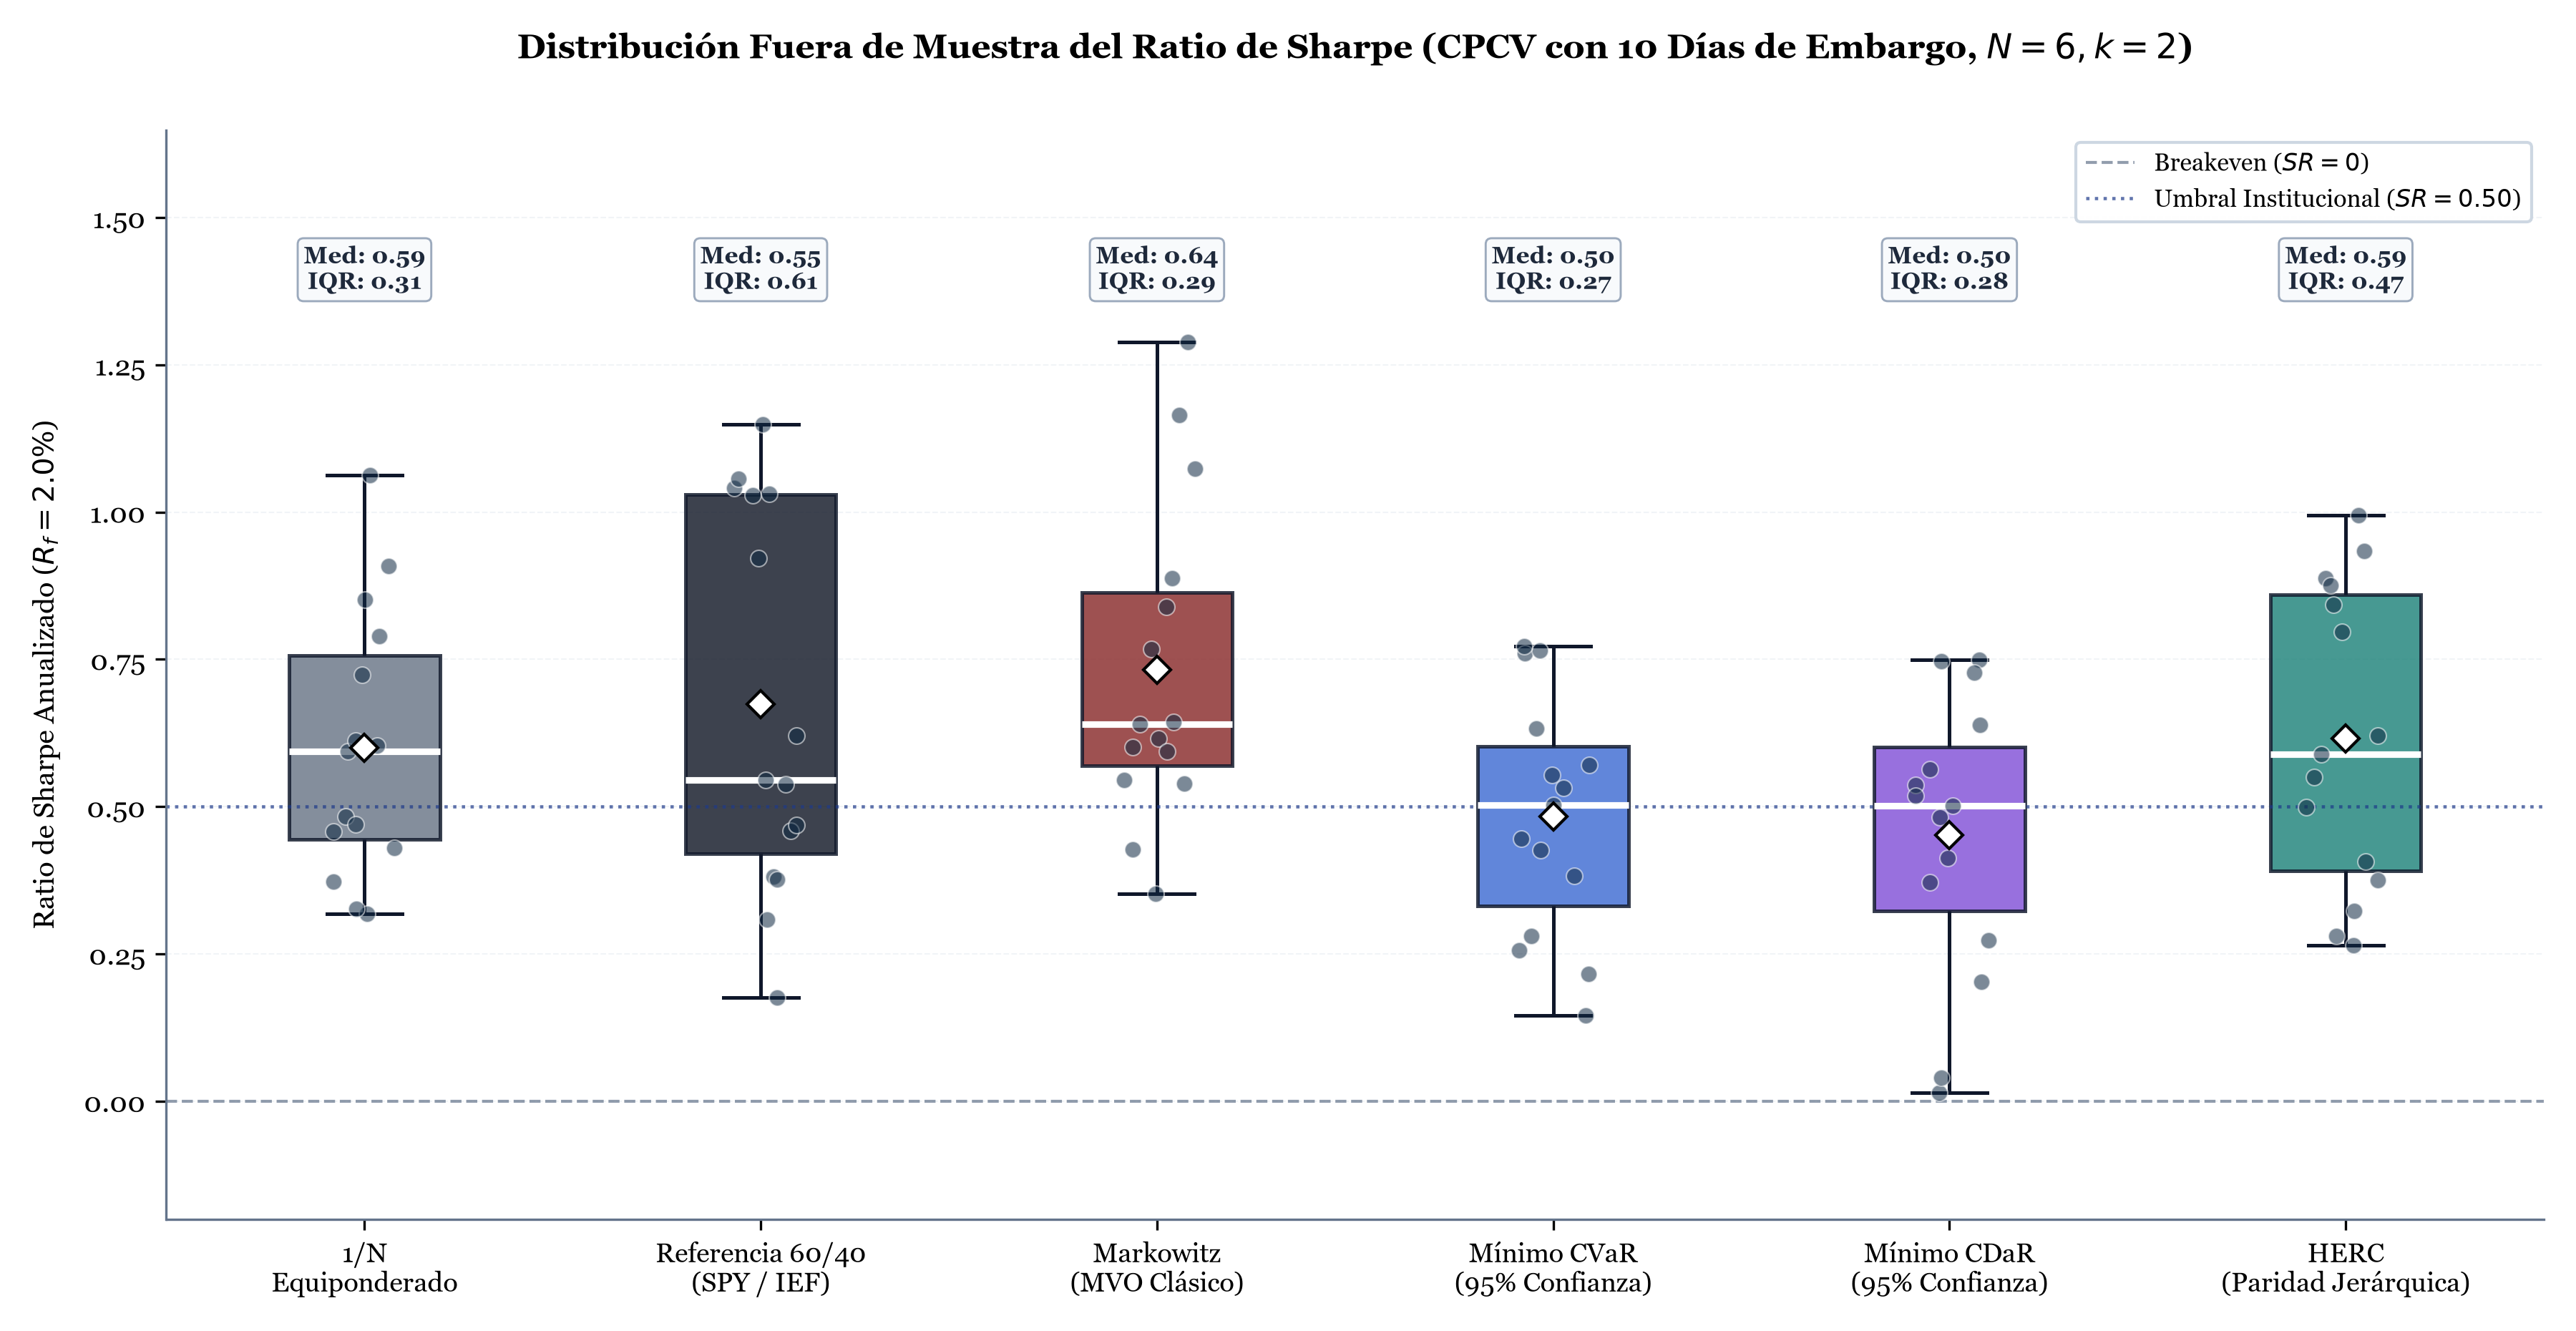
\includegraphics[width=0.86\textwidth]{fig06_cpcv_distribucion_sharpe.png}
\caption{Distribución fuera de muestra del Ratio de Sharpe bajo Validación Cruzada Combinatoria con Embargo (CPCV, 15 particiones independientes, 8 estrategias --incluye DRO-Wasserstein y Mínimo CVaR Ex-Ante, evaluados bajo la misma partición $N=6$, $k=2$).}
\label{fig:cpcv}
\end{figure}

\section{Resultados Empíricos y Análisis Comparativo}

La Tabla~\ref{tab:metricas} presenta el desempeño de las estrategias durante el período de evaluación fuera de muestra (2010--2026), organizada en cuatro bloques temáticos.

\begin{table}[H]
\centering
\renewcommand{\arraystretch}{1.18}
\caption{Indicadores de desempeño, riesgo, colas extremas y operatividad fuera de muestra (2010--2026) para los nueve modelos evaluados en este documento.}
\label{tab:metricas}
\resizebox{\textwidth}{!}{%
\begin{tabular}{lrrrrrrrrr}
\toprule
\textbf{Indicador / Métrica} & \textbf{1/N Equip.} & \textbf{Ref. 60/40} & \textbf{Markowitz} & \textbf{Michaud Rem.} & \textbf{Mín. CVaR} & \textbf{Mín. CDaR} & \textbf{HERC} & \textbf{DRO-Wasserstein} & \textbf{Mín. CVaR Ex-Ante} \\
\midrule
\multicolumn{10}{l}{\textit{\textbf{A. Rendimiento y Retorno Acumulado}}} \\
CAGR (\%) & 7.85 & 9.64 & 11.39 & 10.48 & 5.11 & 5.15 & 6.81 & 7.46 & 4.58 \\
Retorno Acumulado (\%) & 249.2 & 358.5 & 495.6 & 419.9 & 127.9 & 129.3 & 197.2 & 228.7 & 109.8 \\
\midrule
\multicolumn{10}{l}{\textit{\textbf{B. Riesgo y Desempeño Ajustado}}} \\
Volatilidad Anual (\%) & 9.49 & 9.79 & 17.05 & 13.61 & 5.32 & 6.38 & 7.35 & 8.92 & 5.32 \\
Desviación a la Baja (\%) & 10.10 & 10.34 & 18.60 & 14.76 & 5.54 & 6.73 & 7.82 & 9.52 & 5.55 \\
Ratio de Sharpe & 0.617 & 0.781 & 0.551 & 0.623 & 0.584 & 0.493 & 0.654 & 0.612 & 0.485 \\
Ratio de Sortino & 0.580 & 0.739 & 0.505 & 0.575 & 0.561 & 0.468 & 0.615 & 0.573 & 0.465 \\
Ratio de Calmar & 0.376 & 0.455 & 0.290 & 0.368 & 0.314 & 0.265 & 0.323 & 0.356 & 0.258 \\
Ratio de Omega & 1.121 & 1.156 & 1.114 & 1.125 & 1.108 & 1.096 & 1.126 & 1.120 & 1.091 \\
Ratio Ganancia/Pérdida & 1.164 & 1.200 & 1.138 & 1.155 & 1.182 & 1.159 & 1.182 & 1.165 & 1.165 \\
\midrule
\multicolumn{10}{l}{\textit{\textbf{C. Riesgo Extremo y Colas EVT}}} \\
Retroceso Máximo (\%) & -20.86 & -21.18 & -39.32 & -28.48 & -16.29 & -19.39 & -21.11 & -20.93 & -17.78 \\
CDaR 95\% (\%) & -14.77 & -15.52 & -35.61 & -25.49 & -12.77 & -15.81 & -15.35 & -14.90 & -12.78 \\
VaR 95\% Diario (\%) & -0.90 & -0.94 & -1.74 & -1.41 & -0.52 & -0.61 & -0.72 & -0.86 & -0.52 \\
CVaR 95\% Diario (\%) & -1.40 & -1.47 & -2.71 & -2.12 & -0.79 & -0.97 & -1.09 & -1.31 & -0.79 \\
VaR 99\% EVT (\%) & -1.54 & -1.56 & -2.87 & -2.28 & -0.83 & -0.99 & -1.17 & -1.44 & -0.83 \\
CVaR 99\% EVT (\%) & -1.96 & -1.98 & -3.56 & -2.83 & -1.05 & -1.25 & -1.53 & -1.84 & -1.06 \\
Coeficiente de Asimetría & -0.547 & -0.308 & -0.530 & -0.525 & -0.173 & -0.291 & -0.368 & -0.559 & -0.218 \\
Curtosis de Exceso & 9.10 & 9.74 & 4.09 & 4.89 & 3.69 & 5.55 & 7.75 & 9.16 & 4.52 \\
\midrule
\multicolumn{10}{l}{\textit{\textbf{D. Significancia y Operatividad}}} \\
PSR (vs 0) (\%) & 99.34 & 99.92 & 98.67 & 99.39 & 99.09 & 97.70 & 99.58 & 99.30 & 97.53 \\
DSR (\%) & 95.45 & 99.64 & 95.33 & 97.90 & 97.24 & 93.29 & 98.49 & 98.48 & 96.64 \\
Rotación Anualizada (\%) & 0.00 & 0.00 & 288.75 & 503.76 & 66.37 & 261.02 & 31.43 & 3.77 & 413.00 \\
Nº Efectivo de Activos ($N_{\text{eff}}$) & 9.00 & 1.92 & 1.31 & 2.65 & 1.84 & 2.16 & 6.46 & 8.92 & 1.93 \\
\bottomrule
\end{tabular}%
}
\end{table}

La asignación dinámica de capital en cada rebalanceo mensual se detalla en la Figura~\ref{fig:pesos}. Markowitz MVO rota de forma abrupta entre clases de activos (Panel A). HERC mantiene una estructura diversificada y estable (Panel C). DRO-Wasserstein apenas varía en 16 años (Panel E). Mínimo CVaR Ex-Ante reasigna capital de forma abrupta en casi cada rebalanceo (Panel F), la contrapartida visual directa de su rotación de $413.00\%$ en la Tabla~\ref{tab:metricas}. La Figura~\ref{fig:drawdown} presenta las curvas de riqueza acumulada y los episodios de retroceso durante las crisis de 2011, 2020 y 2022 para las nueve estrategias. La descomposición del presupuesto de riesgo frente a la ponderación nominal se muestra en la Figura~\ref{fig:riesgo} (Paneles A--D).

\begin{figure}[H]
\centering

\includegraphics[width=0.98\textwidth]{fig03_evolucion_pesos_walk_forward.png}
\caption{Evolución temporal de la asignación de activos a lo largo de los rebalanceos mensuales fuera de muestra (2010--2026): Markowitz MVO (A), Mínimo CVaR (B), HERC (C), Referencia 60/40 (D), DRO-Wasserstein (E) y Mínimo CVaR Ex-Ante (F).}
\label{fig:pesos}
\end{figure}

\begin{figure}[H]
\centering

\includegraphics[width=0.92\textwidth]{fig04_retorno_acumulado_y_drawdown.png}
\caption{Evolución de la riqueza acumulada (base 100) y curvas de retroceso con identificación de regímenes de crisis (2010--2026). Incluye las nueve estrategias evaluadas en este documento: 1/N, 60/40, Markowitz, Michaud, Mín. CVaR, Mín. CDaR, HERC, DRO-Wasserstein y Mínimo CVaR Ex-Ante.}
\label{fig:drawdown}
\end{figure}

\begin{figure}[H]
\centering

\includegraphics[width=0.92\textwidth]{fig07_descomposicion_riesgo_cluster.png}
\caption{Descomposición del presupuesto de riesgo: Ponderación de capital ($w_i$) frente a Contribución Marginal al Riesgo ($\%RC_i$) por activo. Markowitz MVO (Panel A) y HERC (Panel B) sobre la asignación estática de muestra completa ya reportada en la Sección 3; DRO-Wasserstein (Panel C) y Mínimo CVaR Ex-Ante (Panel D) sobre la misma optimización aplicada una sola vez a toda la muestra, para comparabilidad directa con A y B.}
\label{fig:riesgo}
\end{figure}

\section{Análisis Comparativo por Modelo}

Ningún modelo domina al resto en todas las métricas. Cada estrategia resuelve un problema distinto, con costos y ventajas que dependen del mandato de inversión. A continuación se describe cada uno.

\subsection{Equiponderado (1/N)}

La cartera equiponderada fija $w_i = 1/9$ sin estimar parámetros. No tiene error de estimación y es el único modelo cuya solución no depende de los datos históricos. DeMiguel et al.\ (2009) mostraron empíricamente que 1/N supera a Markowitz en retorno ajustado por riesgo en la mayoría de los conjuntos de datos con ventanas de estimación inferiores a 50 años. Es consecuencia directa de la amplificación del error muestral en el optimizador cuadrático. Alcanza $N_{\text{eff}} = 9.00$, el más alto del universo. Su limitación es estructural: asigna igual capital a activos con volatilidades muy distintas (IEF: 6.9\%; VNQ: 29.6\%).

\subsection{Cartera 60/40}

La cartera 60/40 (60\% SPY, 40\% IEF) registra el mayor CAGR neto (9.64\%), el mejor Sharpe (0.78), el mejor Sortino (0.74) y el DSR más alto (99.64\%). Es la referencia contra la que se comparan los demás modelos y ninguno la supera en retorno ajustado por riesgo dentro del período analizado.

Sus resultados dependen del régimen: el ciclo 2010--2026 estuvo dominado por expansión tecnológica y tasas reales negativas. En la práctica es casi un portafolio de dos activos ($N_{\text{eff}} = 1.92$). En 2022 la correlación positiva entre bonos y acciones produjo una caída del $-21.18\%$, lo que pone de manifiesto que la diversificación entre clases no siempre opera en episodios de contracción simultánea.

\subsection{Markowitz Media-Varianza}

Markowitz MVO registra el mayor retorno acumulado del universo (CAGR 11.39\%, acumulado 495.64\%), pero con el peor perfil de riesgo. La volatilidad anual es de 17.05\%, el retroceso máximo de $-39.32\%$, el $\text{CVaR}_{99\%}^{\text{EVT}}$ de $-3.56\%$ y la rotación anual de 288.75\%. El Sharpe de 0.55 es el más bajo. El retorno adicional frente al 60/40 no compensa el riesgo en ninguna métrica ajustada. La concentración en $N_{\text{eff}} = 1.31$ activos es consecuencia del comportamiento de amplificador de errores (\textit{error maximizer}) documentado por Michaud (1989): errores pequeños en $\hat{\mu}$ se amplifican en las ponderaciones y concentran la cartera en activos con alto retorno histórico reciente.

\subsection{Mínimo CVaR y Mínimo CDaR}

Ambos modelos minimizan medidas de riesgo de cola. El CVaR es una medida coherente (Artzner et al., 1999) que cumple subaditividad, propiedad que la varianza no garantiza en distribuciones asimétricas. El CDaR (Chekhlov et al., 2005) optimiza la trayectoria de retrocesos, es decir, el promedio de los peores episodios bajo el máximo histórico. Min-CVaR registra el menor retroceso máximo ($-16.29\%$), el menor VaR y el menor CVaR de cola de todo el universo.

El costo es el retorno. El CAGR queda en 5.11\%--5.15\% y el acumulado en 127.9\%--129.3\%, por debajo de la cartera 60/40 y del equiponderado. Min-CDaR presenta además rotación elevada (261.02\%) por la sensibilidad de la optimización de trayectorias a cambios en la ventana de estimación. Estos modelos son apropiados cuando el mandato impone un límite duro de pérdida máxima.

\subsection{HERC}

HERC distribuye el presupuesto de riesgo entre clústeres jerárquicos sin estimar retornos esperados. Sus valores fuera de muestra son $N_{\text{eff}} = 6.46$, rotación de 31.43\%, $\text{PSR} = 99.58\%$, $\text{DSR} = 98.49\%$ y $\text{CVaR}_{99\%}^{\text{EVT}} = -1.53\%$.

HERC \textbf{no maximiza el retorno absoluto}. Con CAGR de 6.81\% y retorno acumulado de 197.22\% queda por debajo del 60/40, del equiponderado y de Markowitz MVO. Tampoco minimiza el retroceso, donde Min-CVaR es superior. Lo que HERC logra es un resultado razonable en todas las métricas al mismo tiempo: retorno moderado, retroceso moderado, alta diversificación efectiva y baja rotación.

\subsection{DRO-Wasserstein}

Con $\varepsilon = 0.02$, la penalización de norma $\|w\|_2$ empuja la solución lejos de las concentraciones que favorece el CVaR empírico puro. El resultado es una cartera con $N_{\text{eff}} = 8.92$, prácticamente equiponderada en términos de diversificación efectiva aunque no en pesos nominales, y una rotación anualizada de $3.77\%$, la más baja de \textbf{todos} los modelos evaluados, incluido HERC. El Sharpe ($0.612$) queda entre Mínimo CVaR ($0.584$) y HERC ($0.654$). El DSR ($98.48\%$) confirma que el resultado no es producto del azar de haber evaluado múltiples estrategias. La robustez distribucional no mejora el Sharpe crudo respecto de HERC, pero ofrece el perfil de menor fricción operativa del estudio. Eso es relevante para mandatos con restricciones estrictas de costos de transacción o impacto de mercado. La Figura~\ref{fig:pesos}E confirma visualmente esta estabilidad: la composición por activo apenas varía entre 2010 y 2026. El Panel C de la Figura~\ref{fig:riesgo} muestra además que, a diferencia de Markowitz, ningún activo concentra desproporcionadamente la contribución al riesgo.

\subsection{Marco Generativo Ex-Ante}

El marco generativo ex-ante \textbf{no confirma} la expectativa de la literatura de que reemplazar retornos históricos por escenarios sintéticos GARCH-EVT-cópula mejore el desempeño fuera de muestra. Frente al Mínimo CVaR ex-post, con el mismo nivel de confianza $\alpha=0.95$ y el mismo universo, el Sharpe cae de $0.584$ a $0.485$, el retroceso máximo empeora levemente de $-16.29\%$ a $-17.78\%$ y la rotación anualizada se dispara de $66.37\%$ a $413.00\%$. Eso es un orden de magnitud mayor, comparable a Markowitz MVO ($288.75\%$) o Michaud ($503.76\%$), los dos modelos que este documento identifica como operativamente inviables.

La causa más probable es la siguiente: el pronóstico de un paso adelante $(\mu_{i,t+1}, \sigma_{i,t+1})$ de cada activo es, por construcción, más reactivo mes a mes que un promedio histórico de 756 ruedas. La cartera óptima resultante persigue la volatilidad condicional \textit{vigente} en cada rebalanceo en lugar de una estimación suavizada. Eso genera el mismo patrón de rotación excesiva que Michaud (1989) documenta para el error de estimación muestral en $(\hat{\mu}, \hat{\Sigma})$, aquí trasladado a la dimensión temporal del pronóstico GARCH. Es consistente con la motivación original de HERC/HRP, que busca evitar invertir matrices de covarianza ruidosas, pero aplicada a un problema distinto: pronosticar $\sigma_{t+1}$ con precisión no implica que optimizar directamente contra ese pronóstico, rebalanceo a rebalanceo, sea operativamente estable. La Figura~\ref{fig:pesos}F hace visible el mecanismo: a diferencia de cualquier otro panel de este documento, la composición cambia de forma abrupta rebalanceo a rebalanceo, sin un patrón de tendencia estable.

Esto no invalida el marco generativo ex-ante como herramienta de \textit{medición} de riesgo de cola, el uso para el que la literatura citada en la Subsección \ref{sec:exante} lo diseñó originalmente. Invalida específicamente su uso \textbf{directo} como insumo de un optimizador de Mínimo CVaR con rebalanceo mensual sin alguna forma de suavizado o penalización de turnover, por ejemplo \textit{shrinkage} hacia el pronóstico del período anterior. El resultado se reporta sin ajustes adicionales, en línea con el resto del documento.

\subsection{Comparación vs. cartera 60/40}

La Tabla~\ref{tab:benchmark} resume si cada modelo supera, iguala o queda por debajo del 60/40 en cada dimensión.

\begin{table}[H]
\centering
\renewcommand{\arraystretch}{1.15}
\caption{Posición relativa vs. cartera 60/40. \checkmark: supera; $\circ$: comparable (diferencia relativa $\lesssim 5\%$ o efecto mixto); $\times$: inferior.}
\label{tab:benchmark}
\resizebox{\textwidth}{!}{%
\begin{tabular}{lrrrrrr}
\toprule
\textbf{Métrica} & \textbf{Markowitz MVO} & \textbf{Mín. CVaR} & \textbf{HERC} & \textbf{1/N} & \textbf{DRO-Wass.} & \textbf{Mín. CVaR Ex-A.} \\
\midrule
CAGR (\%) & \checkmark & $\times$ & $\times$ & $\times$ & $\times$ & $\times$ \\
Sharpe & $\times$ & $\times$ & $\times$ & $\times$ & $\times$ & $\times$ \\
Retroceso máximo & $\times$ & \checkmark & $\circ$ & $\circ$ & $\circ$ & \checkmark \\
$\text{CVaR}_{99\%}^{\text{EVT}}$ & $\times$ & \checkmark & \checkmark & $\times$ & $\circ$ & \checkmark \\
Rotación & $\times$ & $\circ$ & \checkmark & \checkmark & \checkmark & $\times$ \\
$N_{\text{eff}}$ & $\times$ & $\times$ & \checkmark & \checkmark & \checkmark & $\circ$ \\
DSR (\%) & $\times$ & $\times$ & $\circ$ & $\times$ & $\circ$ & $\times$ \\
\bottomrule
\end{tabular}%
}
\end{table}

Ningún modelo supera al 60/40 en Sharpe dentro del período analizado, incluidos DRO-Wasserstein y Mínimo CVaR Ex-Ante. Los modelos de colas y HERC tienen sentido cuando el mandato impone restricciones de pérdida o requiere mayor número de activos efectivos, no como alternativa de mayor retorno. DRO-Wasserstein agrega a esa lista el menor costo de rotación del estudio. Mínimo CVaR Ex-Ante es, de los nueve, el único que empeora simultáneamente en rotación y en significancia estadística (DSR) frente a su propio análogo ex-post.

\subsection{Drawdown, Compounding y la Asimetría de las Pérdidas}

Una pérdida del $X\%$ requiere una ganancia de $X/(1-X)$ para recuperar el nivel inicial. Una caída del $-39.32\%$ (Markowitz MVO) exige un retorno bruto de aproximadamente $+64.8\%$ solo para volver al \textit{high-water mark}. Durante ese período de recuperación el capital no se compone hacia adelante. La interrupción del compounding destruye retorno logarítmico acumulado de forma permanente.

Magdon-Ismail y Atiya (2004) formalizaron el retroceso máximo esperado como función del ratio de Sharpe y el horizonte temporal:
\begin{equation}
\mathbb{E}[\text{MaxDD}(T)] \approx \sqrt{\frac{\pi}{2}} \cdot \frac{\sigma_{\text{anual}}}{\text{SR}} \cdot \sqrt{T}
\end{equation}
Dado un Sharpe de 0.55 y $\sigma = 17.05\%$, Markowitz genera retrocesos esperados considerablemente mayores que HERC (Sharpe 0.65, $\sigma = 7.35\%$) en cualquier horizonte.

Grossman y Zhou (1993) demostraron que bajo un mandato de preservación de capital (límite de retroceso), la solución óptima no es la cartera de media-varianza, sino una que gestiona activamente la distancia al máximo histórico. Este resultado justifica formalmente los modelos Min-CDaR y, en menor medida, HERC como alternativas a Markowitz cuando el mandato incluye restricciones de pérdida.

En la teoría del crecimiento óptimo de capital, Vince (1992) demostró que la maximización del crecimiento geométrico ---equivalente al criterio de Kelly--- penaliza el retroceso en forma multiplicativa. Una estrategia con alta tasa de ganancia pero pérdidas profundas puede destruir más capital geométrico que una con menor tasa de aciertos pero pérdidas limitadas. El resultado directo es que controlar la magnitud de la pérdida domina a maximizar la frecuencia de retornos positivos en la función de crecimiento de largo plazo.

\section{Comportamiento en Regímenes de Crisis y Conclusiones}

Los resultados fuera de muestra muestran diferencias cuantitativas entre modelos que no pueden atribuirse a una sola causa.

Durante las crisis de 2011, 2020 y 2022, HERC registró un retroceso máximo de $-21.11\%$, frente a $-39.32\%$ en Markowitz MVO y $-28.48\%$ en Michaud. DRO-Wasserstein ($-20.93\%$) queda en la misma zona que HERC y el 60/40. Mínimo CVaR Ex-Ante ($-17.78\%$) contiene mejor la caída que el resto, aunque no tanto como el propio Mínimo CVaR histórico ($-16.29\%$) que busca reemplazar. En 2022 la correlación positiva entre bonos y acciones afectó al 60/40 ($-21.18\%$), mientras que la ponderación de HERC en materias primas (DBC) y oro (GLD) redujo la caída relativa.

Markowitz MVO acumula el mayor retorno fuera de muestra (495.64\%), por encima del 60/40 (358.51\%), DRO-Wasserstein (228.66\%) y HERC (197.22\%). Este resultado se explica por la concentración en renta variable tecnológica durante un ciclo favorable para esa clase de activos. Ese retorno se obtiene con el mayor retroceso del universo ($-39.32\%$) y el Sharpe más bajo (0.55): el riesgo adicional asumido no fue compensado proporcionalmente.

Markowitz MVO rota a 288.75\% anual y Michaud a 503.76\%. HERC opera a 31.43\% y DRO-Wasserstein a 3.77\%, la rotación más baja de las nueve estrategias. Mínimo CVaR Ex-Ante es la excepción que confirma que la rotación no depende solo de la robustez matemática del modelo: con 413.00\% anual, su reasignación mensual es tan agresiva como la de Michaud, pese a partir de un marco de calibración de colas más sofisticado que el resto del documento. Markowitz concentra el capital en $N_{\text{eff}} = 1.31$ activos. HERC alcanza $N_{\text{eff}} = 6.46$, con $\text{PSR} = 99.58\%$, $\text{DSR} = 98.49\%$ y $\text{CVaR}_{99\%}^{\text{EVT}} = -1.53\%$ frente a $-3.56\%$ de Markowitz; DRO-Wasserstein llega a $N_{\text{eff}} = 8.92$, la diversificación efectiva más alta entre los modelos que sí estiman parámetros (solo 1/N, que no estima nada, la supera).

Ningún modelo de los nueve domina en todas las dimensiones. Las dos incorporaciones más recientes no cambian esa conclusión. DRO-Wasserstein es la que mejor complementa a HERC en este universo: misma familia de resultados moderados, pero con la menor fricción operativa del estudio, relevante para mandatos sensibles a costos de transacción. El Marco Generativo Ex-Ante, en cambio, no traslada su rigor de calibración de colas a una mejora de desempeño cuando se lo usa como insumo directo del optimizador. Sharpe (0.485) y rotación (413.00\%) quedan peor posicionados que el propio Mínimo CVaR histórico que busca reemplazar. El resultado se reporta sin ajustar porque el objetivo de este documento es la evidencia empírica, no la confirmación de la hipótesis de partida.

\section{Limitaciones del Estudio y Extensiones Metodológicas}

El modelo asume ejecución a precios de cierre ajustados. En activos de menor profundidad de mercado, como DBC o VNQ, los costos reales intradiarios pueden superar la cota de 5 puntos básicos.

La calibración de la distribución GPD requiere un número suficiente de observaciones en la cola ($n > 50$). El filtrado GARCH(1,1) de McNeil y Frey (2000) estandariza los excesos purgando los efectos ARCH. Sin embargo, el empleo de ventanas rodantes rectangulares (756 ruedas) impone cierta inercia temporal ante cambios abruptos de régimen. Como extensiones metodológicas naturales, la integración de modelos de cambio de régimen de Markov (Hamilton, 1989; Ang y Bekaert, 2002) y matrices de correlación condicional dinámica (DCC; Engle, 2002; Patton, 2006) permitirían modular dinámicamente las probabilidades de transición entre estados de mercado. Ambas quedan como trabajo futuro.

El universo de 9 ETFs permanece constante durante todo el horizonte temporal para aislar las diferencias algorítmicas, sin considerar altas o bajas de activos en el tiempo.

\section*{Bibliografía}
\addcontentsline{toc}{section}{Bibliografía}
\begingroup
\sloppy
\setlength{\leftskip}{1.25em}
\setlength{\parindent}{-1.25em}
\small

Ang, A., \& Bekaert, G. (2002). Regime switches in interest rates. \textit{Journal of Business \& Economic Statistics}, 20(2), 163--182.

Artzner, P., Delbaen, F., Eber, J. M., \& Heath, D. (1999). Coherent measures of risk. \textit{Mathematical Finance}, 9(3), 203--228.

Balkema, A. A., \& de Haan, L. (1974). Residual life time at great age. \textit{The Annals of Probability}, 2(5), 792--804.

Barone-Adesi, G., Giannopoulos, K., \& Vosper, L. (1999). VaR without correlations for nonlinear portfolios. \textit{Journal of Futures Markets}, 19(5), 583--602.

Chekhlov, A., Uryasev, S., \& Zabarankin, M. (2005). Drawdown measure in portfolio optimization. \textit{International Journal of Theoretical and Applied Finance}, 8(1), 13--58.

Chopra, V. K., \& Ziemba, W. T. (1993). The effect of errors in means, variances, and covariances on optimal portfolio choice. \textit{The Journal of Portfolio Management}, 19(2), 6--11.

DeMiguel, V., Garlappi, L., \& Uppal, R. (2009). Optimal versus naive diversification: How inefficient is the 1/N portfolio strategy? \textit{The Review of Financial Studies}, 22(5), 1915--1953.

Demarta, S., \& McNeil, A. J. (2005). The $t$ copula and related copulas. \textit{International Statistical Review}, 73(1), 111--129.

Engle, R. F. (1982). Autoregressive conditional heteroscedasticity with estimates of the variance of United Kingdom inflation. \textit{Econometrica}, 50(4), 987--1007.

Engle, R. F. (2002). Dynamic conditional correlation: A simple class of multivariate generalized autoregressive conditional heteroskedasticity models. \textit{Journal of Business \& Economic Statistics}, 20(3), 339--350.

Esfahani, P. M., \& Kuhn, D. (2018). Data-driven distributionally robust optimization using the Wasserstein metric: Performance guarantees and tractable reformulations. \textit{Mathematical Programming}, 171(1--2), 115--166.

Grossman, S. J., \& Zhou, Z. (1993). Optimal investment strategies for controlling drawdowns. \textit{Mathematical Finance}, 3(3), 241--276.

Hamilton, J. D. (1989). A new approach to the economic analysis of nonstationary time series and the business cycle. \textit{Econometrica}, 57(2), 357--384.

Jarque, C. M., \& Bera, A. K. (1980). Efficient tests for normality, homoscedasticity and serial independence of regression residuals. \textit{Economics Letters}, 6(3), 255--259.

Ledoit, O., \& Wolf, M. (2004). A well-conditioned estimator for large-dimensional covariance matrices. \textit{Journal of Multivariate Analysis}, 88(2), 365--411.

López de Prado, M. (2014). The Deflated Sharpe Ratio: Correcting for selection bias, backtest overfitting, and non-normality. \textit{The Journal of Portfolio Management}, 40(5), 94--107.

López de Prado, M. (2016). Building diversified portfolios that outperform out of sample. \textit{The Journal of Portfolio Management}, 42(4), 59--69.

López de Prado, M. (2018). \textit{Advances in Financial Machine Learning}. John Wiley \& Sons.

Magdon-Ismail, M., \& Atiya, A. F. (2004). Maximum drawdown. \textit{Risk Magazine}, 17(10), 99--102.

Markowitz, H. (1952). Portfolio selection. \textit{The Journal of Finance}, 7(1), 77--91.

McNeil, A. J., \& Frey, R. (2000). Estimation of tail-related risk measures for heteroscedastic financial time series: An extreme value approach. \textit{Journal of Empirical Finance}, 7(3--4), 271--300.

McNeil, A. J., Frey, R., \& Embrechts, P. (2015). \textit{Quantitative Risk Management: Concepts, Techniques and Tools} (Revised Edition). Princeton University Press.

Merton, R. C. (1980). On estimating the expected return on the market: An exploratory investigation. \textit{Journal of Financial Economics}, 8(4), 323--361.

Michaud, R. O. (1989). The Markowitz optimization enigma: Is 'optimized' optimal? \textit{Financial Analysts Journal}, 45(1), 31--42.

Patton, A. J. (2006). Modelling asymmetric exchange rate dependence. \textit{International Economic Review}, 47(2), 527--556.

Patton, A. J. (2012). A review of copula models for economic time series. In G. Elliott \& A. Timmermann (Eds.), \textit{Handbook of Economic Forecasting} (Vol.~2, pp. 89--145). Elsevier.

Pickands, J. (1975). Statistical inference using extreme order statistics. \textit{The Annals of Statistics}, 3(1), 119--131.

Raffinot, T. (2017). Hierarchical clustering-based asset allocation. \textit{The Journal of Portfolio Management}, 44(2), 89--99.

Raffinot, T. (2018). The hierarchical equal risk contribution portfolio. \textit{Financial Markets and Portfolio Management}, 32(2), 241--261.

Rockafellar, R. T., \& Uryasev, S. (2000). Optimization of conditional value-at-risk. \textit{Journal of Risk}, 2(3), 21--42.

Rockafellar, R. T., \& Uryasev, S. (2002). Conditional value-at-risk for general loss distributions. \textit{Journal of Banking \& Finance}, 26(7), 1443--1471.

Vince, R. (1992). \textit{The Mathematics of Money Management: Risk Analysis Techniques for Traders}. John Wiley \& Sons.

\endgroup

\end{document}

